\chapter{Android Application}
\section{Einleitung}
Um eine höchst mögliche Reichweite an Endgeräten zu erzielen, wurde eine Android Applikation entwickelt, mit der die wichtigsten Funktionen abgedeckt werden. Zum Beispiel das Wechseln der DataSets des Digital Signage Servers. Wichtig war es die Applikation möglichst einfach und leicht bedienbar zu gestalten, um auch Erstbenutzern die Bedienung zu erleichtern. 
Prototyp für die aktuelle Applikation war eine Anwendung für Android, die direkt mit dem Digital Signage Server kommuniziert, da sehr schnell klar wurde, dass das Steuern des Servers direkt über eine Applikation auf Android Basis viel zu umständlich ist, wurde eine weitere Mobile Applikation entwickelt, welche über das ''HomeDsBackend''(Java-EE-Server) kommuniziert, um das Funktionsspektrum zu erweitern und die Applikation möglichst kompakt zu gestalten. Beispielsweise ist es durch diese Aufteilung nicht mehr nötig eine Datenbank in der Applikation zu haben. Somit erleichtert es auch Applikationen für andere Betriebssysteme zu implementieren. 
\section{Anforderungen}
Die Anforderungen an die Android Applikation weichen von den Anforderungen an das ''Backend'' leicht ab, da das ''Backend'' die gesamte Zeitsteuerung- und Datenbankfunktionalität übernimmt. Es besteht die Möglichkeit, den Server über die Website des ''Backend'' zu steuern, beziehungsweise über die Applikation auf Android Basis. 
\begin{itemize}
	\item {\em Eilmeldungen:} Dem Benutzer soll es möglich sein Nachrichten in einem Ticker auf den Bildschirmen anzuzeigen.
	
	\item {\em Medien Wiedergabe:} Medien die Lokal am Digital Signage Server liegen sollen abgespielt werden können.
		
	\item {\em Authentifizierung automatisieren (Prototyp Applikation):} Die Authentifizierung am Digital Signage Server soll automatisiert werden, um nicht vom Benutzer durchgeführt werden zu müssen.  		
\end{itemize}
\section{Verwendete Technologien}
\subsection{Android}
Android wird mit der API(Englisch: application programming interface / Deutsch: Anwendungsprogrammierschnittstelle), in der Version 26 (Oreo / Android 8.0) verwendet. 
VERWEIS ANDROID !!!!
\subsection{OkHttp3}
Als Erweiterung für die Http Anfragen an den Digital Signage Server und das HomeDsBackend wird OkHttp3 verwendet.
\section{Struktur}
\begin{itemize}
	\item {\em activity:} Alle Activities die für die Anwendung benötigt werden. Als Beispiel die MainActivity
	
	\item {\em adapter:} Hier befinden sich alle Adapter für die RecyclerViews.
	
	\item {\em apiClient:} Beinhaltet die Klasse ''RequestHelper'' mit der die Anfragen an den Digital Signage Server beziehungsweise an das HomeDsBackend vereinfacht werden.
	
	\item {\em entity:} Jene Klassen die als Models für die Anwendung benötigt werden. 
	STÜTZ!!!
	
	\item {\em enumeration:} Enumerationen welche die Android Basierte Applikation verwendet. Zum Beispiel das ''RequestTypeEnum''.
	
	\item {\em fragment:} Alle Fragments die für das User Interface benötigt werden. Beispiel hierfür ist das Fragment ''NewsOverviewFragment'', welches alle DataSets die am Server sind anzeigt.
	
	\item {\em viewholder:} Beinhaltet alle ''ViewHolder'' die für die Verschiedenen ''RecyclerViews'' benötigt werden. 		
\end{itemize}
\section{Benutzerhandbuch}
\subsection{Startseite}
Auf der Einstiegsseite der Applikation ist ein Feld mit dem Serverstatus zu sehen sollte dieses Rot eingefärbt sein gibt es Verbindungsprobleme zum Server(die Applikation kann keine Daten vom Server erhalten oder Daten an den Server senden) andernfalls kann mit der Benutzung fortgefahren werden. Die Funktion der Beiden Buttons wird im weiteren velauf des Benutzerhandbuchs erklärt.
\\
Bild Rot und Grün
\\
\subsection{Abspielen von Medien auf gewünschten Bildschirmen}
Das Abspielen von Medien wird im Navigationstab ''Play Media'' abgewickelt, des weiteren befindet sich auf der Startseite ein Button über den direkt zu dieser Sektion navigiert werden kann.
\\
\begin{mediaNav}
\centering
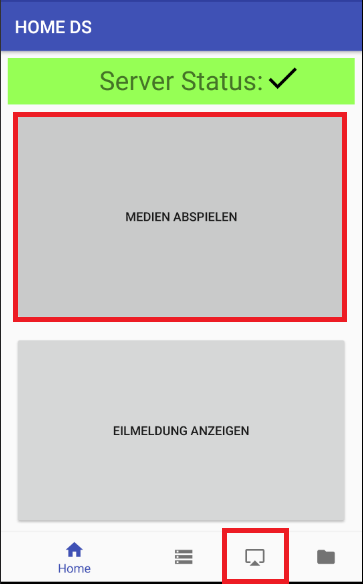
\includegraphics[width=1.0\textwidth]{images\06_AndroidApp\06_mediaNavigation}
\caption{Startseite mit markierten Navigationselementen}
\label{fig:mediaNav}
\end{mediaNav}
\\
Wurde noch kein Display gewählt, auf dem das Medium abgespielt werden soll, erscheint zu beginn eine Auswahlmaske für die Bildschirme die verfügbar sind. Nach Auswahl einer Anzeige navigiert die Applikation automatisch zur Medienübersicht. Ist bereits ein Bildschirm ausgewählt wird direkt eine Übersicht der abspielbaren Medien angezeigt. Im rechten oberen Teil der Ansicht ist der Gewählte Bildschirm zu sehen und über einen Button wird die Bildschirmauswahl angezeigt.
\\
\begin{dispChoi}
\centering
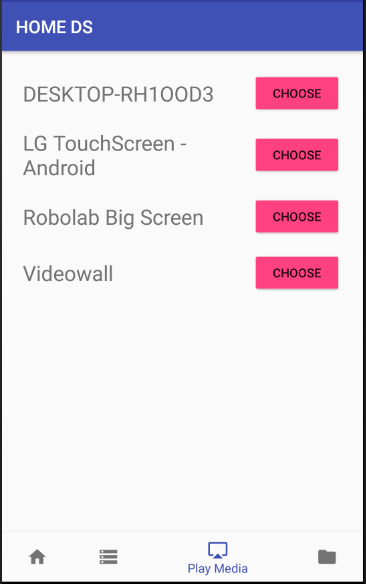
\includegraphics[width=1.0\textwidth]{images\06_AndroidApp\06_displayChoice}
\caption{Liste mit verfügbaren Displays}
\label{fig:mediaNav}
\end{dispChoi}
\\
\begin{dispBut}
\centering
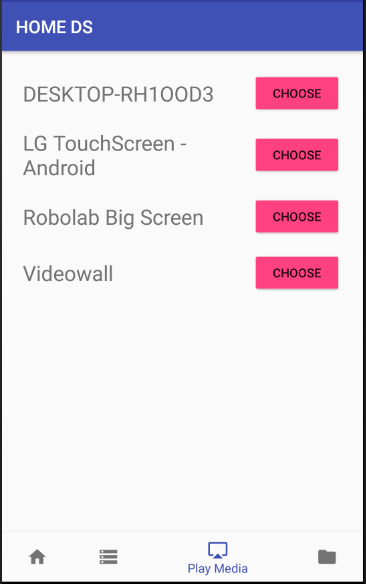
\includegraphics[width=1.0\textwidth]{images\06_AndroidApp\06_displayChoice}
\caption{Ausgewählter Bildschirm und Button für die Auswahl}
\label{fig:mediaNav}
\end{dispBut}
\\
Sortieren der angezeigten Medien ist über einen Spinner im linken oberen Teil der Medien Übersicht möglich durch Berührung der Anzeigefläche erscheint die Auswahl der Sortiervorschläge.
\begin{tagSpinn}
\centering
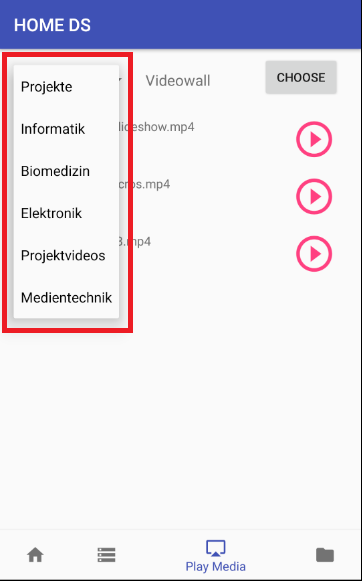
\includegraphics[width=1.0\textwidth]{images\06_AndroidApp\06_TagChoice}
\caption{Spinner mit Tags zur Sortierung}
\label{fig:mediaNav}
\end{tagSpinn}
\\
Um ein in der Liste angezeigtes Medium abzuspielen muss der Play-Button im rechten teil des Listenelements gedrückt werden. Wurde der Button betätigt wird das Medium auf der gewählten Anzeige abgespielt.
\begin{playBut}
\centering
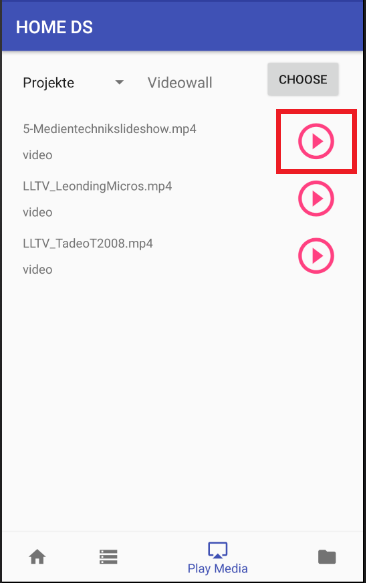
\includegraphics[width=1.0\textwidth]{images\06_AndroidApp\06_playMedia}
\caption{Play Button um Medium abzuspielen}
\label{fig:mediaNav}
\end{playBut}
\\
\subsection{Meldungen Anzeigen}
Um eine Meldung anzuzeigen muss zum ''DataSet'' Tab gewechselt werden dies ist auch über eine Schaltfläche auf der Startseite von statten gehen.
\begin{navDataSet}
\centering
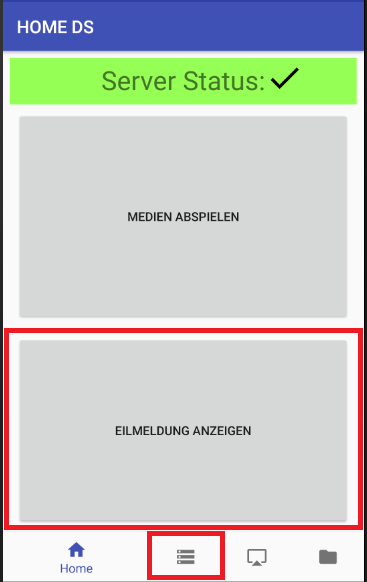
\includegraphics[width=1.0\textwidth]{images\06_AndroidApp\06_dataSetNavigation}
\caption{Startseite mit Navigationselementen}
\label{fig:mediaNav}
\end{navDataSet}
\\
Die im der Ansicht zu sehende Liste enthält alle aktiven und  inaktiven Meldungen die auf den Anzeigen wiedergegeben werden beziehungsweise werden können. 
\\
Bild 
\\
Durch auswählen eines der Listenelemente öffnet sich einer Detailansicht über die die Informationen der Meldung verändert werden können zum Beispiel der Titel oder der Anzeigezeitraum. Wird der FloatingActionButton im unteren rechten teil der Ansicht gedrückt so öffnet sich ein Detailfenster welches noch keine Daten eingetragen hat um eine neue Meldung zu erstellen.
\\
Bild
\\
Vorgenommene Änderungen oder neu erstellte Meldungen können mittels Save Button übernommen werden. Dieser befindet sich im unteren teil der Detailansicht. Nach speichern einer Meldung navigiert die Applikation wieder auf die Übersicht der Meldungen.
\\
Bild
\\
\subsection{Strukturübersich}
Ist es von Nöten eine detailierte Übersicht über die am Server liegenden Layouts zu bekommen kann dies über den Navigationstab ''Structure Plan'' getan werden. 
\\
Bild navigatin
\\
Die Liste zeigt alle am Server befindlichen Layouts durch klicken einer der Listenelemente navigiert die Applikation zu einer Detailansicht des Layouts.
\\
bild click element
\\
Die Detailansicht eines Layouts zeigt die Grunddaten eines Layouts wie zum Beispiel die ID oder die Besitzer ID. Des weiteren werden alle unterelemente beispielsweise Widget's angezeigt. Dargestellt wird der JSON-String des Layouts.
\\
Bild detail
\\
\section{MainBottomNavigationActivity und OverveiwFragment}
\subsection{MainBottomNavigationActivity}
Die ''MainBottomNavigationActivity'' ist die Einzige ''Activity'' die in der Android Applikation benötigt wird. Hauptaufgabe der ''MainBottomNavigationActivity'' ist es, zwischen den einzelnen ''Fragments'' zu navigieren. Enthalten sind dazu jene Methoden, welche mit dem ''SupportFragmentManager'' die einzelnen Fragments im ''container\_main'' austauschen. Der ''container\_main'' ist ein ''ConstraintLayout'' welches in der zur ''MainActivity'' gehörenden Layout Ressource ''activity\_main.xml'' mit der Identifikationsnummer ''container\_main'' und  belegt wurde. Zudem wird die Klasse durch das Interface ''AppCompatActivity'' erweitert und implementiert die ''OnFragmentInteractionListener'' der Fragmente die in der Applikation verwendet werden. 
\
Im unteren Teil der ''Activity'' befindet sich eine Navigationsleiste. Diese ist zuständig für das wechseln zwischen den einzelnen Fragmenten mit folgenden Navigationspunkten: 

\begin{itemize}
	\item {\em Home:} Jener Menüpunkt der die Startseite der Applikation beinhaltet.
	\item {\em DataSet:} Ist zuständig für die Verwaltung der ''DataSets''.
	\item{\em Medium abspielen:} Beinhaltet die Fragmente die benötigt werden um Medien auf der gewünschten anzeige abzuspielen.
	\item {\em Strukturplan:} Bietet eine Übersicht über die Struktur der am Server liegenden Layouts.
\end{itemize}
\subsubsection{onCreate}
Hier wird die ''MainBottomNavigationActivity'' als ''ContentView'' gesetzt, zudem wird mittels ''SupportFragmentManager'' das ''HomeScreenFragment'' dem ''container\_main'' zugewiesen und angezeigt. Die statische Variable ''instance'', vom Datentyp ''MainBottomNavigationActivity'', wird auf die aktuelle Instanz der Klasse zugewiesen. 	
\subsubsection{getInstance}
 Ist der ''Getter'' für die statische Variable ''instance'' und übergibt die aktuelle Instanz der Klasse.
\subsubsection{Fragment-austausch-Methoden}
 Sind jene Methoden die für das Austauschen der einzelnen ''Fragments'' im ''container\_main'' zuständig sind. Dies geschieht mittels ''SupportFragmentManager'' welcher immer die ''Fragments'' im ''container\_main'' anzeigt und dem ''BackStack'', welcher für die Rückwerts Navigation (mittels retour Knopf des Mobilen Endgerätes) in der Applikation zuständig ist,  hinzufügt. Manche Methoden übergeben zudem noch ein ''Bundle'' an das erstellte ''Fragment'', welches Objekte enthält die in nächsten ''Fragment'' benötigt werden. Erkennungsmerkmal dieser Methoden ist das englische Verb ''open'' am beginn des Methodennamens. Als Namensbeispiel hierfür wird die Methode ''openNewsEditFragment'' herangezogen.
\subsection{HomeScreenFragment}
Der Einstiegspunkt der Applikation ist das ''HomeScreenFragment''. Es zeigt den Serverstatus an, dieser wird über einen ''REST-Request'' vom Java-EE-Server abgefragt. Den Hauptanteil des Fragments bilden die beiden Navigations-Buttons ''Median abspielen'' und ''Eilmeldungen anzeigen''. Durch klicken dieser Buttons öffnen sich die dazugehörigen Fragmente ''NewsOverviewFragment'' und ''MediaOverviewFragment''.
\\
Die Layout Ressource des ''HomeScreenFragment'' enthält zwei Buttons und ein ''ConstaintLayout''. Dieses ''ConstraintLayout'' beinhaltet wiederum eine ''TextView'' und zwei ''ImageViews''. In der ''onCreate'' Methode des Fragments werden als erstes die Anzeigeelemente neu deklarierten Variablen zugewiesen und im ''ConstraintLayout'' wird der Serverstatus auf View standardmäßig als Offline angezeigt und die Buttons deaktiviert. Im folgenden Schritt wird über einen ''GET-Request'' die Uhrzeit des XIBO-Servers über den Java-EE-Server abgefragt. Wird eine Uhrzeit vom erhalten, so wird im ''ConstraintLayout'' des Server Status auf online gesetzt und das dazugehörige Bild angezeigt und die Buttons werden freigegeben. Erhält man keine Antwort bleibt die Anzeige unverändert.
\section{DataSet Verwaltung}
Die beiden Fragmente  ''NewsOverviewFragment'' und ''NewsEditFragment'' sind für die Verwaltung der ''DataSets'' zuständig. Im Fragment ''NewsOverviewFragment'' wird eine Übersicht über alle vorhandenen ''DataSets'' gegeben. Das ''NewsEditFragment'' Fragment wird verwendet um vorhandene ''DataSets'' zu bearbeiten oder neue ''DataSets'' zu erstellen. 
\subsubsection{NewsOverviewFragment}
Dieses Fragment zeigt alle aktiven ''DataSets'' an, diese werden vom Server bereitgestellt und per ''REST-Request'' abgefragt. Über einen ''FloatingActionButton'' kann ein neues ''DataSet'' erstellt werden. Durch klicken auf eines der Listen Elemente, öffnet sich eine Detailansicht in der das Bearbeiten, eines des ''DataSets'' möglich ist.
\\
Die Layout Ressource des Fragments, ''fragment\_news\_overview.xml'' enthält eine ''RecyclerView'' und einen ''FloatingActionButton''. Die Logik der Anzeige ist in der Java Klasse ''NewsOverviewFragment'' implementiert. Die meisten Methoden dieser Klasse werden generisch beim Erstellen eines Fragments erzeugt. Die einzige Methode die überschrieben wurde ist die Methode ''onCreateView''. Beim Ausführen dieser Methode wird zuerst eine ''View'' erstellt welche das ''fragment\_news\_overview'' Layout zugewiesen bekommt. Anschließend wird eine ''RecyclerView'' und ein ''FlaootingActionButton'' erstellt und den zugehörigen Anzeige Elementen zugewiesen. Der ''FlaootingActionButton'' erhält einen ''OnClickListener'' über diesen wird in der ''MainActivity'' eine Methode aufgerufen die ein neues ''NewsEditFragment'' anzeigt, um ein neues ''DataSet'' zu erstellen. 
\subsubsection{NewsEditFragment}
Das Fragment zeigt alle Details eines ''DataSets'' an und bietet die Möglichkeit die Detailinformationen bearbeiten zu können. Ebenso wird dieses Fragment dazu verwendet, ein neues ''DataSet'' zu erstellen, dazu wird das Fragment mit Hinweisen auf die Eingabeoptionen erstellt. Über einen Button können die eingegeben Felder an den ''Java-EE-Server'' übermittelt werden. Eingabe Felder:
\begin{itemize}
	\item {\em Titel:} Das Feld ''Titel'' beinhaltet die Überschrift der anzuzeigenden Information.
	\item {\em Beschreibung:} Hier wird der eigentliche Informationstext eingefügt.
	\item{\em Datum-Von-Bis:} Diese Felder werden über ein ''DatePickerDialog'' befüllt, welcher einen Kalender öffnet und zeigen an in welchen Zeitraum das ''DataSet'' angezeigt wird. 
	\item {\em Uhrzeit-Von-Bis:} Die anzeige Elemente geben Auskunft über die Zeitspanne in der das ''DataSet'' an den einzelnen Tagen angezeigt wird. Das Feld kann mittels ''TimePickerDialog'' befüllt werden.		
\end{itemize}
Anzeige Ressourcen für dieses Fragment werden in der Datei ''fragment\_news\_edit.xml'' bereitgestellt. Diese enthält die benötigten Tags, um die im oberen Teil beschrieben Eingabefelder zur Verfügung zu stellen. Die Verwendung und Belegung dieser Felder wird in der Klasse ''NewsEditFragment'' implementiert. Auch in dieser Klasse wurde nur die Methode ''onCreateView'' mit Quellcode versehen. Zu Beginn wird der deklarierten ''View'' die ''fragment\_news\_edit.xml'' als Ressource zugewiesen. Um Daten aus dem ''NewsOverviewFragment'' zu empfangen wird ein ''Bundle'' befüllt. Wenn das befüllte ''Bundle'' Informationen beinhaltet, dann wird die Funktion ''setArguments'' der Basisklasse Fragment(android.support.v4.app.Fragment) mit dem Parameter ''bundle'' aufgerufen, um das Feld ''mArguments'' der Basisklasse Fragment mit Daten zu versehen(Vererbung). Die zuvor deklarierten Variablen (benötigte ''Views'') werden jetzt initialisiert. Das Fragment hat zwei verschiedene Vorgehensweisen. Zum einen werden, sollte ein ''DataSet'' in Form eines ''Bundels'' übergeben werden, die Anzeigeelemente mit den übergebenen Werten befüllt. Andernfalls werden die Felder mit keinen Werten versehen, es werdend Hinweise auf die Eingabeoptionen im aktuellen Fragment angezeigt. Die benötigten ''onClickListener'' für die Datums und Uhrzeit eingaben werden im Anschluss implementiert und mittels ''DatePickerDialog'' beziehungsweise ''TimePickerDialog'' mit Daten versehen. Durch Drücken des Buttons(Speicher Button) wird ein Event ausgelöst. Dieses Event kann zwei verschiedene Ausgänge haben: Wenn das im Event erhaltene ''Bundle'' eine ''ID'' besitzt, lässt sich daraus eindeutig schließen, ob es sich hierbei um ein Dataset handelt, das vom User erstellt wurde, oder um eines, das bereits zuvor am Java-EE-Server vorhanden war, indem man überpfrüft, ob die im Bundle enthaltene Information ''ID'' den Wert null hat, oder nicht. Falls dies nämlich der Fall ist, sind es eindeutig vom Benutzer eingegebene Daten. Somit muss deswegen am Server anschließend ein ''POST-Request'' durchgeführt werden, um die neu erstellten Informationen zu senden.
Wenn es ein vom Java-EE-Server erhaltenes ''DataSet'' ist, wird stattdessen ein ''PUT-Request'' durchgeführt, der die veränderten Daten übermittelt.  
\section{Mediaplayer}
Um auf einer gewünschten Anzeige ein, sich auf dem Server befindliches, Medium abzuspielen wurden die beiden Fragments ''MediaOverViewFragment'' und ''ChooseDisplayFragment'' implementiert. Das gewünschte Medium wird auf dem ausgewählten Display sofort Abgespielt. Ist noch kein Display ausgewählt wird man zuerst auf das ''ChooseDisplayFragment''gelitet um einen anzeige Display zu wählen.
\subsubsection{MediaOverviewFragment}
Im diesem Fragment werden alle Medien angezeigt, die sich am XIBO-Server in der Bibliothek befinden und mit dem Richtigen Tag markiert sind. Eine Sortierung der Liste ist über ein ''Spinner'' Element möglich. Des weiteren wird im rechten oberen teil des Fragments der Display angezeigt auf dem das gewählte Medium abgespielt werden soll. Eine Auswahl des Displays ist über Navigation zum ''ChooseDisplayFragment'' möglich, dieses wird über den Button ''Auswählen'' geöffnet. Hat der Benutzer noch keinen keinen Display ausgewählt wird er zuerst auf das ''ChooseDisplayFragment'' weitergeleitet.
\\
Durch die Ressource Datei ''fragment\_media\_overview.xml'' können die Elemente in der View angezeigt werden. Dieses Layout beinhaltet neben einer ''RecyclerView'' zur Darstellung der abzuspielenden Medien, zwei Buttons eine TextView und einen Spinner zur Sortierung der angezeigten Liste. Einstiegspunkt der Methode ''onCreateView'' ist die zuweisung der Layout Ressource. Weiters werden die in der Klasse deklarierten Variablem mit den Anzeigeelementen verknüpft. Die Textview wird im Anschluss mit dem Namen des, für die Wiedergabe gewählten, Displays belegt. Um die Liste der Medien nach nach belieben zu sortieren wird ein ArrayAdapter initialisiert. Diesem werden die Ressourcen ''tag\_array'', beinhaltet eine Liste mit Sortiermöglichkeiten für die angezeigten Medien, und ''simple\_spinner\_item'' um das Design für die angezeigten ''Spinner'' Elemente, übergeben. Es erfolgt eine Zuweisung des Adapters an das Spinner Element. Um die Sortierung der Medien Liste zu realisieren wird ein ''OnItemSelectedListener'' implementiert der die Medien gefiltert nach ausgewähltem Tag anzeigt. Um zu beginn alle inhalte anzizeigen wird dem Spinner das erste Element des ''tag\_array'' als Standardsortierung zugewiesen. Um zwischen den Einzelnen Displays zu wählen wird dem ''Auswählen'' Button ein ''onClickListener'' zugewiesen welcher die Navigation zum ''ChooseDisplayFragment'' einleitet. Des weiteren wurde die Methode ''setRecyclerView'' erstellt um die Daten nach Tag sortiert vom Server mittels ''GET-Request'' zu erhalten und diese auf der View anzeigen zu können.
\subsubsection{ChooseDisplayFragment}
Die Auswahl des Bildschirmes auf dem das Medium angezeigt werden soll erfolgt über dieses Fragment. Dazu werden die verfügbaren Displays vom Java-EE-Server abgefragt und in einer Liste angezeigt. Durch klicken auf den ''Aüswählen'' Button in einem der in der Liste angezeigten Display Elementen, wird dieser Display ausgewählt und Medien werden dann auf diesem Abgespielt. 
\\
Die RecyclerView Ressource um die zu wählenden Displays anzuzeigen ist in der Datei ''fragment\_choose\_display.xml'' angelegt. Zuweisen der Layout ressource auf die aktuelle View, initialisieren der Klassen Attribute und aufrufen der Methode ''getDisplays'' sind die einzigen Schritte der ''onCreateView'' Funktion.''getDisplays'' ist jene Methode die alle Displays die mit dem XIBO-Server verbunden sind per ''GET-Request'' abfragt beziehungsweise aufbereitet und der RecyclerView übergibt um diese auf der View anzuzeigen. 
\section{Strukturplan}
Die am XIBO-Server liegenden Layouts werden in der Andoid Applikation formatiert als ''JSON-Sting'' angezeigt. Damit ist gewährleistet, dass der App-Benutzer eine Übersicht über die Struktur der einzelnen Layouts und deren Unterelemente zur Verfügung hat.
\subsubsection{StructurePlanFragment}
Dieses Fragment zeigt eine Übersicht der einzelnen Layouts in Form einer Liste an. Durch klicken der einzelnen Listen Elemente navigiert die Applikation zu einer Detailansicht über das gewählte Layout.
Die Ressource zur gestaltung der Anzeige beinhaltet eine ''RecyclerView'' und heißt ''fragment\_structure\_plan.xml''. Zu beginn der ''onCreateView'' Methode wird zuerst eine ''View'' erstellt welche das ''fragment\_structure\_plan.xml'' Layout zugewiesen bekommt. Die ''RecyclerView'' wird anschließend initialisiert und über einen ''GET-Request'', dessen Response die einzelnen Layouts und deren unterstrukturen,des Xibo-Servers in form eines JSON-Strings übermittelt, befüllt. Somit ist auf der Anzeige eine Liste mit auswählbaren Layouts vorhanden über die zu einer Detailansicht navigiert werden kann. 
\subsubsection{StructureDetailFragment}
Ein Layout wird in diesem Fragment in Form eines ''JSON-Strings'' mit allen dazugehörigen Unterelementen angezeigt. Wichtig hierbei ist es den Angezeigten ''JSON-String'' richtig zu formatieren um die Übersichtlichkeit bei zu behalten.
\\
In der Ressource Datei ''fragment\_structure\_detail.xml'' befindet sich eine ''TextView'' als einziges Element. Die ''onCreateView'' Methode der Klasse ''StructureDetailFragment'', wird nach zuweisen der Layout Ressource der Struktur beschreibende ''JSON-String'' aus dem ''Bundle'' gelesen, dies geschieht über die Methode ''setArguemnts'' der Basisklasse Fragment und deren Feld ''mArguments'', und dem Anzeigefeld zugewiesen. Anschließend wird dem Fragment noch die fähigkeit gegeben sich Scrollen zu lassen und die View wird zurückgegeben. 
\section{Request-Helper}
Um in weiterer Folge die Anfragen an den Java-EE-Server einfach und einheitlich durchzuführen gibt es die Klasse ''RequestHelper'' . In dieser Klasse gibt es neben den beiden Parametern ''responseBody'' und ''responseCode'', welche zur Fehlerausgabe und zum Erhalt der Daten aus der Anfrage vorhanden sind, die Methode ''executeRequest''. Diese übernimmt die Hauptaufgabe der Klasse und führt die Anfragen an das Signage System durch. Werden Daten als Antwort der anfrage erwartet so kann die Methode mit ''Callback'' Parameter aufgerufen werden, ist dies nicht der Fall so gibt es die Möglichkeit diese Methode ohne ''Callback'' aufzurufen, dabei wird dieser Parameter mit dem Wert null überschrieben.
\\
Die Parameter dieser Methode lauten wie folgt:
\\
\begin{itemize}
	\item {\em RequestTypeEnum:} Der Parameter vom Typ Enum wird genutzt um Herauszufinden welche Http Anfrage vorliegt. Mögliche Werte sind hierbei GET, POST, PUT und DELETE.
	
	\item {\em Params:} Hier liegt eine HashMap vor, die als Key-Value Paare alle benötigten Parameter für den RequestBody beinhaltet. Beispielsweise: ''LayoutID'':''78'', hierbei ist ''LayoutID'' der Key und ''78'' das Value.
		
	\item {\em Url:} Beinhaltet die URL unter der die Anfrage erreichbar ist. 
	
	\item {\em Callback:} Dieser Parameter wird benötigt, um auf eine Antwort des ausgeführten ''REST-Request'' zu warten. Wird ein ''Response'' erhalten und die Daten werden in dem angezeigten Fragment benötigt, können diese über eine ''Lamda-Expression'' in die gewünschten Anzeigeelemente eingefügt werden. 
\end{itemize}
Zu Beginn der Methode wird anhand des Parameters RequestTypeEnum unterschieden, um welche Http Anfrage es sich handelt. Wird GET oder DELETE geliefert wird durch die HashMap iteriert und die einzelnen Key-Value Paare als QeryParameter in der URL einfügt.
Beispielsweise:''<URL>/layout?layoutID=78'' .
\\
Handelt es sich um eine POST oder PUT Anfrage so werden die Key-Value Paare im Body mitgegeben und im Format "application/x-www-form-urlencoded" codiert, andernfalls werden die Parameter als ''Query-Parameter'' übergeben, Anschließend wird die URL mittels HttpUrl.Builder erstellt und ausgegeben. 
Des Weiteren wird per Switch-Case dem Request die richtige Art der Anfrage zugewiesen und danach die URL übergeben. 
\\
Um die REST-Anfragen fertig zu stellen, wird das Interface Callback implementiert. Mit den beiden Methoden onFailure und onResponse wird dem Interface zugewiesen was passiert, wenn der Request fehlschlägt oder funktioniert. 
\\
\textbf{onFailure:}
Sollte der Request fehlschlagen, wird im Log-Fenster der Responsecode und die Fehlermeldung/Exception ausgegeben. 
\textbf{onResponse:}
Wird der Request ohne Fehler durchgeführt so wird im Log-Fenster ebenfalls der Responsecode und der Responsebody ausgegeben. Letzter schritt beim Erhalt des gewünschten ''Response'' ist es dem im Methoden Kopf übergebenen ''Callback'' Parameter auszuführen, dieser enthält zum Beispiel siehe Abbildung.
Bild!!!!!!!!!!!
\\
Der letzte Schritt ist es dem OkHttpClient mitzuteilen, dass er einen neuen Call ausführen soll. Als Parameter wird der Zusammengestellte Request mitgegeben. Über .enqueue wird dem Client gesagt er soll auf einen Response warten. Parameter für diese Methode ist das erstellte Interface Callback.
\cite{OkHttp3}
\\
Um Daten aus den Requests zu erhalten beziehungsweise Fehlerausgaben anzeigen zu können gibt es Getter zu den Feldern ''responseBody'' und ''responseCode''. Verläuft der Request fehlerfrei so werden die geforderten Werte in die variablen übertragen und können im weiteren verlauf durch die Methoden ''getResponseCode'' beziehungsweise ''getResponseBody'' (Getter) ausgelesen werden. Im Fehlerfall wird lediglich der ''responseCode'' mit dem Fehlercode belegt und kann ausgelesen werden. 
\\
Antworten des Servers werden in Form von JSON-Strings erhalten. Das Aufbereiten dieser Daten wird den Einzelnen Fragmenten, welche die Anfragen in Auftrag geben, überlassen, da die Erhaltenen Informationen von Fragment zu Fragment verschiedene Inhalte aufweisen. 
\\
Um klarzustellen wie das Aufbereiten der Daten von statten geht wird anhand des Beispiels ''StructurePlanFragment'' gezeigt was passiert sollte die Anfrage eine positive Antwort erhalten. Zu beachten ist, dass die Zuweisung der erhaltenen Daten in einer Lamda-Expression durchgeführt wird. Als erstes werden eine Liste von JSON-Objekten und ein JSONArray deklariert, um das Anzeigen und Durchlaufen der Informationen zu ermöglichen. Das Array wird hierbei zum Durchlaufen benötigt. Die LinkedList bildet die Quelle für die Anzeigedaten des Fragments. Da JSON-Strings im Folgenden Abschnitt geparst werden ist ein try-catch block nötig in dem Mögliche Fehlerfälle behandeln und ausgegeben zu können. Die übermittelten Daten werden über den ''responseBody'' Getter ausgelesen und in das JSONArray übernommen. Über Iteration durch das JSONArray werden die einzelnen JSONObjekte ausgelesen und der LinkedList angehängt. Nicht immer ist eine Iteration durch den Erhaltenen JSON-String nötig, beispielsweise bei der Anfragen in der der XIBO-Server-Status festgestellt wird. Im Anschluss werden die Anzeigeelemente mit den ausgelesenen Werten versehen, dabei ist zu beachten, dass dieser schritt über den UI-Thread ausgeführt wird da nach erzeugen der View die Anzeigeelemente verändert werden. 
\\